\documentclass{article}
\usepackage[utf8]{inputenc}
\usepackage[english]{babel}
\usepackage{graphicx}
\usepackage{float}
\usepackage{listings}
\usepackage{hyperref}
\usepackage{amsmath}
\hypersetup{
    colorlinks=true,
    linkcolor=blue,
    filecolor=magenta,      
    urlcolor=cyan,
}
\urlstyle{same}

\title{Manual 3 - 2do Torneo de Programación Competitiva}
\author{Lions R.C.}
\date{Julio 2019}

\begin{document}

\maketitle

\tableofcontents

\begin{figure}[H]
    \centering
    
\includegraphics[width=0.2\paperwidth]{newblack}
\end{figure}

\section{Estructuras de datos avanzadas}

Hasta ahorita solo hemos visto estructuras de datos sencillas (vectores, pares, mapas y sets) que tienen el proposito de guardar valores de una manera conveniente para su acceso. Ahora se verán estructuras que guardan valores en cierta orden o configuración con el fin de simplificar programas más avanzadas.

\subsection{Stack}

El stack o la pila en español es una estructura de datos que, como indica su nombre, apila datos desde abajo hasta arriba. El concepto detrás de esta estructura es igual al de la vida real; si tienes una caja donde vas apilando hojas, debes sacar la hoja que esta hasta arriba antes de que puedas sacar la que esta debajo de esa y viceversa.

Digamos que tenemos 6 enteros, {6, 5, 2, 9, 3} y los insertamos en nuestra pila empezando con 6 y terminando con 3. Nuestra pila se verá de la siguiente manera:

\begin{figure}[H]
    \centering
    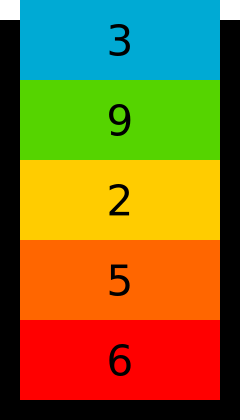
\includegraphics[width=0.1\paperwidth]{pila}
\end{figure}

Debido a la implementación interna de la pila, no podemos sacar un valor que este debajo de otro sin sacar todos los de arriba primero. Esta propiedad se llama \textbf{LIFO} en íngles o Last In First Out (el último en entrar es el primero en salir).

Si ahora sacamos todos los valores y los guardamos en un arreglo, veremos que se invertió el orden de los datos debido a esta propiedad: {3, 9, 2, 5, 6}.

Para incluir una pila en C++, se llama la librería \textbf{stack} y se declara con sintaxis \textbf{\lstinline{stack<tipo> nombre;}}.

Para agregar objetos a una pila, se puede utilizar la función \textbf{push(valor)} y para eliminar el dato que esta hasta arriba se debe hacer \textbf{pop()}. Para ver el dato que esta hasta arriba se puede utilizar \textbf{top()} y para ver cuantos elementos tiene se puede llamar a \textbf{size()}.

Vamos a crear un programa que invierte los valores que originalmente habiamos visto:

\begin{lstlisting}[language=C++, caption=Pilas]
#include <iostream>
#include <stack>

using namespace std;

int main() {
    stack<int> pila;
    int valores[] = {6, 5, 2, 9, 3};
    for(int i = 0; i < 5; i++) {
        pila.push(valores[i]);
    }
    while(pila.size() > 0) {
        cout << pila.top() << endl;
        pila.pop();
    }
}
\end{lstlisting}
\href{https://repl.it/@Jamesscn/Cargando-pilas}{Liga al código} \\

Como se puede observar al correr el programa, los valores se imprimen al revés.

La pila no solo sirve para invertir cosas, sino que es util para cuando quieres procesar los datos más recientes antes que las más antiguas.

Digamos que estas diseñando el buzón de un red social como Facebook o Twitter y tu quieres enseñarle a tus usuarios las publicaciones más recientes, pero también quieres eliminar las publicaciones vistas por el usuario para que no tengan que desplazarse mucho para ver más contenido.

Esto se puede implementar con una pila que va apilando las publicaciones más recientes y cada vez que el usuario se desplaza para abajo se quitan las publicaciones que estan hasta arriba.

\subsection{Queue}

El queue o la fila es en cierto sentido el complemento de la pila. La fila, como también indica el nombre, funciona como una fila de datos donde el primero en entrar es el primero en salir. Esto se llama \textbf{FIFO} en íngles o First In First Out.

\begin{figure}[H]
    \centering
    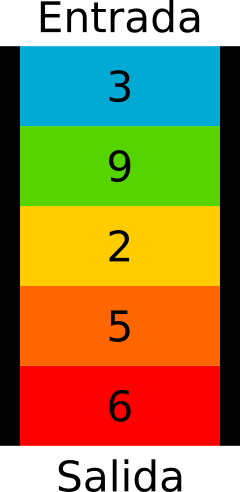
\includegraphics[width=0.1\paperwidth]{fila}
\end{figure}

Como se puede observar, los datos estan haciendo fila y saldrían en el mismo orden de la que entran, no se invierten. Al igual que una pila, un valor que esta hasta atrás no puede salir primero.

Para implementarlo, se debe incluir la librería \textbf{queue} y se debe declarar como \textbf{\lstinline{queue<dato> nombre;}}.

Las funciones de esta estructura son algo distintos a las de la pila. Para insertar y quitar datos, se puede utilizar \textbf{push(valor)} y \textbf{pop()} respectivamente, pero para ver el valor que esta hasta en frente se debe llamar \textbf{front()}. Como támbien tiene una parte de atrás, este se puede ver con \textbf{back()}.

\begin{lstlisting}[language=C++, caption=Filas]
#include <iostream>
#include <queue>

using namespace std;

int main() {
    queue<int> fila;
    int valores[] = {6, 5, 2, 9, 3};
    for(int i = 0; i < 5; i++) {
        fila.push(valores[i]);
    }
    while(fila.size() > 0) {
        cout << fila.front() << endl;
        fila.pop();
    }
}
\end{lstlisting}
\href{https://repl.it/@Jamesscn/Haciendo-filas}{Liga al código} \\

Esta estructura es bastante útil debido a que ahorra memoria al borrar datos que ya no ocupa y permite hacer una especie de buffer o vector que almacena datos que no se pueden procesar uno por uno.

Un ejemplo de la fila es cuando quieres promover un producto tuyo a muchas personas. Puedes empezar promoviendole a un amigo tuyo y preguntandole si tiene amigos que le interesa tu producto, luego preguntas a cada uno de esos amigos por sus amigos y sigues repitiendo el proceso hasta haber promovido tu producto a una cantidad satisfactoria de gente.

La pila junto con la fila se aplicarán en las semanas que siguen para resolver problemas relacionados a grafos, como encontrar la respuesta a un laberinto o averiguar el camino más rápido entre dos ciudades.

\subsection{Deque}

El deque es una estructura especial debido a que puede funcionar como pila y fila a la vez. El nombre deque viene del termino double ended queue en íngles o fila con dos salidas.

Se llama de esta manera debido a que funciona como una pila porque puedes insertar datos y luego sacar el primer dato que fue ingresado, y además puedes sacar el último dato que fue ingresado.

\begin{figure}[H]
    \centering
    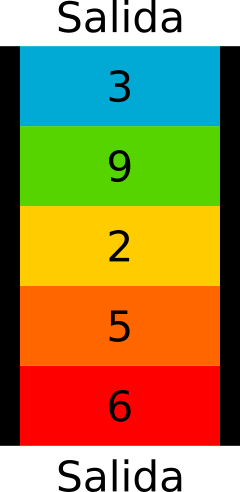
\includegraphics[width=0.1\paperwidth]{deque}
\end{figure}

Si usamos este ejemplo, no podemos obtener los valores de en medio, pero sí podemos sacar el 3 o el 6. Si quitamos el 3, ahora podríamos quitar el 9 o el 6.

Para implementar un deque, se debe incluir la librería \textbf{deque} y se puede crear con \textbf{\lstinline{deque<tipo> nombre;}}

El deque fue implementado de una manera más flexible que las otras estructuras, y sí te permite ver los datos que están en su interior. Para guardar un dato en la parte de enfrente o quitar un dato, se pueden usar \textbf{\lstinline{push_front(valor)}} y \textbf{\lstinline{pop_front(valor)}} respectivamente, y para guardar datos en la parte de atrás de debe llamar \textbf{\lstinline{push_back(valor)}} y \textbf{\lstinline{pop_back()}}.

Se debe notar que el valor en frente es la que se encuentra en la posición 0 y el valor de atrás es la que está en la posición $N - 1$.

Para ver o modificar algún valor se puede usar el sintaxis de un arreglo, como \textbf{nombre[índice]}. Para ver el valor que esta hasta enfrente o hasta atrás, es recomendable utilizar \textbf{front()} y \textbf{back()}. Para insertar o eliminar valores existen las funciones \textbf{insert()} y \textbf{erase()}.

Un ejemplo práctico del deque es para determinar si una palabra es palindromo. Se puede insertar la palabra en el deque y luego se puede comparar el carácter de enfrente con el de atrás e irlos sacando de dos en dos hasta que quede cero o un valor en el deque.

\begin{lstlisting}[language=C++, caption=Deques]
#include <iostream>
#include <deque>

using namespace std;

int main() {
    string palindromo = "aibofobia";
    deque<char> dobleFila;
    //insertar a la fila
    for(int i = 0; i < palindromo.length(); i++) {
        dobleFila.push_back(palindromo[i]);
    }
    bool valido = true;
    while(dobleFila.size() > 1) {
        if(dobleFila.front() != dobleFila.back()) {
            valido = false;
            break;
        }
        dobleFila.pop_front();
        dobleFila.pop_back();
    }
    if(valido) {
        cout << palindromo << " es un palindromo" << endl;
    } else {
        cout << palindromo << " no es un palindromo" << endl;
    }
}
\end{lstlisting}
\href{https://repl.it/@Jamesscn/Deque}{Liga al código}

\subsection{Priority queue}

El priority queue es una especie de fila con prioridad como indica el nombre. Este guarda los valores como una fila normal, pero el primero en salir siempre será el valor mas grande en la fila.

Por ejemplo, un hospital usaría una fila de prioridad para atender sus pacientes, atendiendo al paciente más urgente primero.

Para usar este tipo de dato, se incluye la librería \textbf{queue} igual que cuando se estaba usando una fila y se declara con \textbf{\lstinline{priority_queue<tipo> nombre;}}

Las funciones de este tipo son \textbf{push(valor)} y \textbf{pop()} para agregar o quitar valores y \textbf{top()} para ver el valor que esta enfrente de la fila.

Un ejemplo de estos sería un programa que ordena un arreglo de números flotantes.

\begin{lstlisting}[language=C++, caption=Filas de prioridad]
#include <iostream>
#include <queue>

using namespace std;

int main() {
    float valores[] = {2.22, 3.56, 1.9, 9.52, 3.42, 6.78, 0.11, 4.5};
    priority_queue<float> fila;
    for(int i = 0; i < 8; i++) {
        fila.push(valores[i]);
    }
    for(int i = 0; i < 8; i++) {
        cout << fila.top() << endl;
        fila.pop();
    }
}
\end{lstlisting}
\href{https://repl.it/@Jamesscn/Prioridades}{Liga al código} \\

Esta estructura es muy parecida a un heap, que guarda el dato más grande sobre los demás valores.

\section{Recursividad}

Imaginemos que encontraste un código extraño que parece correr una función dentro de esa misma función. Antes de llamarse a si mismo imprimirá hola y después imprimirá mundo.

\begin{lstlisting}[language=C++, caption=Funciones]
#include <iostream>

using namespace std;

void funcion() {
    cout << "hola" << endl;
    funcion();
    cout << "mundo" << endl;
}

int main() {
    funcion();
}
\end{lstlisting}

Si piensas en la lógica de este programa, tu función correrá, imprimirá "hola" y se correrá denuevo, volviendo a repitir este proceso. Lo que estarias haciendo es crear un ciclo infinito donde tu función corre una copia de esa función que corre otra copia de esa función y nunca se parará.

Si pruebas el código, verás que se imprime hola muchisimas veces hasta que el programa arroja un error. Este error pasa porque cada vez que se llama la función se esta ocupando memoria y llega a un punto donde ya no hay espacio para más funciones. También te darás cuenta que mundo nunca se imprime porque cada función que se llama nunca termina.

Este funcionamiento tiene muchas aplicaciones, por ejemplo, si decidimos correr la función con un parametro entero y decidimos restarle uno a ese número hasta que llegue a 0, podemos calcular la suma de todos los enteros naturales de 1 a N:

\begin{lstlisting}[language=C++, caption=Suma de enteros]
#include <iostream>

using namespace std;

int suma(int n) {
    if(n <= 0) {
        return 0;
    }
    return n + suma(n - 1);
}

int main() {
    cout << suma(100) << endl;
}
\end{lstlisting}

Si analizamos el código, suma con una entrada N primero checará si n es menor o igual a cero, y si no cumple con estas condiciones (es positivo), entonces regresa N + suma(N - 1). Si probamos esto con N = 3, se verá que suma(3) = 3 + suma(2) = 3 + (2 + suma(1)) = 3 + (2 + (1 + suma(0))) = 3 + (2 + (1 + 0)) = 3 + 2 + 1 + 0.

Podemos ver que gradualmente se van sumando los números empezando con N hasta llegar a 0, luego este se regresa en la función original. Cada llamada de suma(N) depende del valor de suma(N - 1).

A esto se le llama la recursividad y es útil para resolver problemas que dependen de un estado anterior. Otro ejemplo de la recursividad es para calcular el factorial de un número; se puede empezar con un número N y multiplicarle N - 1 hasta llegar a 1.

\begin{lstlisting}[language=C++, caption=Factorial recursivo]
#include <iostream>

using namespace std;

long long int factorial(long long int n) {
    if(n <= 1) {
        return 1;
    }
    return n * factorial(n - 1);
}

int main() {
    cout << factorial(10) << endl;
}
\end{lstlisting}

Pero donde brilla la recursividad es en problemas de combinatoria y permutaciones. Si quisieras escribir todas las permutaciones de los caracteres "ABCD", se puede escribir un programa sencillo que explora todas las posibilidades.

\begin{lstlisting}[language=C++, caption=Permutaciones]
#include <iostream>
#include <vector>

using namespace std;

void permutacion(vector<char> letras, vector<char> usadas, int largo) {
    if(usadas.size() == largo) {
        for(int i = 0; i < usadas.size(); i++) {
            cout << usadas[i];
        }
        cout << endl;
        return;
    }
    for(int i = 0; i < letras.size(); i++) {
        usadas.push_back(letras[i]);
        permutacion(letras, usadas, largo);
        usadas.pop_back();
    }
}

int main() {
    vector<char> letras = {'a', 'b', 'c', 'd'};
    vector<char> usadas;
    permutacion(letras, usadas, 5);
}
\end{lstlisting}
\href{https://repl.it/@Jamesscn/Permutando}{Liga al código} \\

Si probamos este código, se imprimirán todas las permutaciones de abcd con 5 letras, empezando con \textbf{aaaaa} y terminando con \textbf{ddddd}. El vector letras contiene las letras que queremos permutar y el vector usadas se va llenando con todas las permutaciones.

\begin{figure}[H]
    \centering
    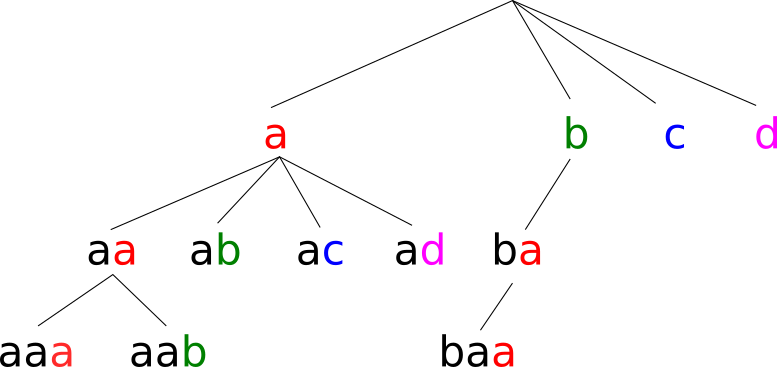
\includegraphics[width=0.3\paperwidth]{permutacion}
\end{figure}

Tenemos un caso donde el vector usadas es igual al largo que queremos, en ese caso imprimimos las letras en ese vector, y si no lo que se hace es que se agregan todas las letras de 'a' a 'd'. Este código en cierto sentido navega un arbol de posibilidades, la primera letra tiene 4 posibilidades, y de esas 4 posibilidades hay 4 posibilidades que le siguen para la siguiente letra. Si calculamos el número total de caminos, obtenemos que es $4^5$ o 1024 permutaciones.

\section{Ordenamientos}

En muchos problemas verás que es más conveniente o más rápido ordenar datos. Existen varios algoritmos de ordenamiento con varias ventajas y desventajas.

\subsection{Ordenamiento por selección}

Este tipo de ordenamiento tiende a ser conocido como "selection sort" en íngles y es fácil de programar con la desventaja que es muy lento (tiene complejidad de tiempo O($N^2$)).

Este método busca el valor más bajo y lo intercambia con el valor en el primer lugar, luego busca el siguiente valor más bajo y lo intercambia con siguiente lugar hasta que se ordena todo el arreglo.

Por ejemplo, si tenemos el arreglo {5, 2, 3, 9, 6} y lo queremos ordenar con este método, intercambiaremos 2 con 5 para obtener {2, 5, 3, 9, 6}. Como sabemos que 2 era el valor más bajo, el arreglo antes del 5 esta ordenado y lo podemos ignorar. Esto significa que ahora solo tenemos que ordenar {5, 3, 9, 6}. Podemos ver que el valor más bajo es 3 y lo podemos intercambiar con el primer lugar para obtener {3, 5, 9, 6}. Nuestro arreglo original es ahora {2, 3, 5, 9, 6}.

Despues solo tendriamos que ordenar {5, 9, 6}, pero como 5 ya esta en el primer lugar podemos saltarnos ese valor y ordenar {9, 6}. Al intercambiar estos valores, obtendriamos el arreglo ordenado {2, 3, 5, 6, 9}.

Este método puede ser implementado con dos ciclos for, uno que va de 0 a N y otro que va del valor actual a N. El segundo ciclo buscará el valor mas bajo de los valores que faltan de ordenarse y el primer ciclo lo ira poniendo en su lugar correcto.

\begin{lstlisting}[language=C++, caption=Ordenamiento por selección]
#include <iostream>

using namespace std;

int main() {
    int valores[] = {5, 2, 3, 9, 6};
    for(int i = 0; i < 5; i++) {
        //Encuentra el valor mas pequeno de i a N
        int indiceMinimo = i;
        for(int j = i; j < 5; j++) {
            if(valores[j] < valores[indiceMinimo]) {
                indiceMinimo = j;
            }
        }
        //Si el valor esta en el primer lugar, ignoralo
        if(indiceMinimo == i) {
            continue;
        }
        //Intercambia los dos valores
        int intercambio = valores[i];
        valores[i] = valores[indiceMinimo];
        valores[indiceMinimo] = intercambio;
    }
    for(int i = 0; i < 5; i++) {
        cout << valores[i] << endl;
    }
}
\end{lstlisting}
\href{https://repl.it/@Jamesscn/Ordenamiento-de-seleccion}{Liga al código} \\

Como se puede observar, su complejidad es de O($N^2$) porque tiene dos ciclos for anidados que van de 0 a N en el peor de los casos.

\subsection{Ordenamiento por mezcla}

Támbien conocido como \textbf{merge sort} en íngles, este tipo de ordenamiento es muy rápido debido a que su complejidad es O($N log N$). Este algoritmo se basa en lo que se llama "Divide y vencerás", esencialmente convierte un problema en más problemas pequeños pero más faciles. Como sigue este modelo tiene una fase de división y parte el arreglo en mitades hasta llegar a un solo elemento. Como un solo elemento ya esta ordenado, se puede juntar con otro arreglo de tamaño uno viendo cual de los dos es más pequeño y poniendo ese primero. Cuando se hace esto, se tendran varios arreglos ordenados con dos elementos, y estos se vuelven a juntar para hacer arreglos ordenados de cuatro elementos y asi sucesivamente.

\begin{figure}[H]
    \centering
    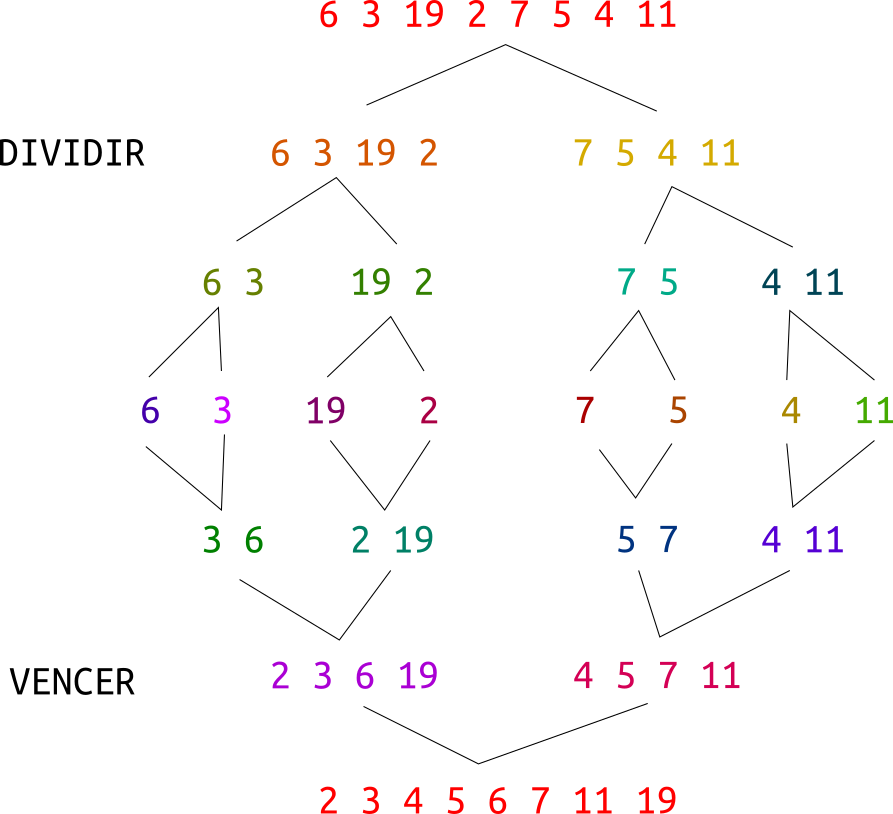
\includegraphics[width=0.4\paperwidth]{mergesort}
\end{figure}

Digamos que queremos ordenar los valores {6, 3, 19, 2, 7, 5, 4, 11}. Partimos los arreglos a la mitad y ahora nos enfocamos en ordenar {6, 3, 19, 2} y {7, 5, 4, 11}. Después decidimos partir estos a la mitad y enfocarnos en ordenar los arreglos {6, 3}, {19, 2}, {7, 5} y {4, 11}. Los partimos una última vez para tener {6}, {3}, {19}, {2}, {7}, {5}, {4}, {11}.

Como habiamos partido {6, 3} para obtener {6} y {3}, podemos juntarlos para hacer un nuevo arreglo ordenado escogiendo el más pequeño de los dos primero: {3, 6}. Al repetir esto con los otros arreglos, se obtiene {3, 6}, {2, 19}, {5, 7}, {4, 11}. Como antes queríamos ordenar {6, 3, 19, 2} y tenemos los dos subarreglos {3, 6} y {2, 19}, podemos formar el arreglo ordenado de cuatro elementos volviendo a escoger el más pequeño de los dos arreglos en cada momento y poniendo ese primero. Al quedarse {2, 3, 6, 19} y {4, 5, 7, 11}, se pueden volver a juntar estos arreglos para tener el arreglo original ordenado.

La manera más sencilla de implementar este algoritmo es usando la recursividad:

\begin{lstlisting}[language=C++, caption=Ordenamiento por mezcla]
#include <iostream>

using namespace std;

void ordenar(int* valores, int tamano) {
    if(tamano < 2) {
        return;
    }
    int mitadA = tamano / 2;
    int mitadB = tamano - mitadA;
    int valoresA[mitadA];
    int valoresB[mitadB];
    for(int i = 0; i < mitadA; i++) {
        valoresA[i] = valores[i];
    }
    for(int i = 0; i < mitadB; i++) {
        valoresB[i] = valores[i + mitadA];
    }
    ordenar(valoresA, mitadA);
    ordenar(valoresB, mitadB);
    int indiceA = 0;
    int indiceB = 0;
    while(indiceA < mitadA && indiceB < mitadB) {
        if(valoresA[indiceA] < valoresB[indiceB]) {
            valores[indiceA + indiceB] = valoresA[indiceA];
            indiceA++;
        } else {
            valores[indiceA + indiceB] = valoresB[indiceB];
            indiceB++;
        }
    }
    while(indiceA < mitadA) {
        valores[indiceA + indiceB] = valoresA[indiceA];
        indiceA++;
    }
    while(indiceB < mitadB) {
        valores[indiceA + indiceB] = valoresB[indiceB];
        indiceB++;
    }
}

int main() {
    int cantidad;
    cin >> cantidad;
    int valores[cantidad];
    for(int i = 0; i < cantidad; i++) {
        cin >> valores[i];
    }
    ordenar(valores, cantidad);
    for(int i = 0; i < cantidad; i++) {
        cout << valores[i] << endl;
    }
}
\end{lstlisting}
\href{https://repl.it/@Jamesscn/Ordenamiento-de-mezcla}{Liga al código}

\subsection{Ordenamiento estandar de C++}

Para ahorrar tiempo y evitar tener que volver a escribir ordenamientos como el de mezcla, C++ tiene una librería que incluye su propia implementación eficiente de ordenamiento. Este ordenamiento se llama \textbf{csort} y tiene complejidad de tiempo O($N log N$).

Para utilizar este ordenamiento, se tiene que incluir la librería \textbf{algorithm}. Luego, se debe llamar la función \textbf{sort()} con dos parámetros, el primer lugar en memoria del arreglo y el ultimo lugar del arreglo. Para un arreglo normal, se puede dar el nombre del arreglo como el primer parámetro y el nombre del arreglo sumado con su tamaño como el segundo parámetro.

\begin{lstlisting}[language=C++, caption=Ordenamiento estandar para un arreglo]
#include <iostream>
#include <algorithm>

using namespace std;

int main() {
    int valores[] = {6, 3, 19, 2, 7, 5, 4, 11};
    sort(valores, valores + 8);
    for(int i = 0; i < 8; i++) {
        cout << valores[i] << endl;
    }
}
\end{lstlisting}

Para vectores y otras estructuras definidas en librerias, se debe usar las funciones \textbf{begin()} y \textbf{end()}

\begin{lstlisting}[language=C++, caption=Ordenamiento estandar para un vector]
#include <iostream>
#include <algorithm>
#include <vector>

using namespace std;

int main() {
    vector<int> valores = {6, 3, 19, 2, 7, 5, 4, 11};
    sort(valores.begin(), valores.end());
    for(int i = 0; i < valores.size(); i++) {
        cout << valores[i] << endl;
    }
}
\end{lstlisting}

Si se desea ordenar un arreglo de una manera especial como ordenar pares por su primer valor, se puede crear una función que maneja el ordenamiento y se le puede pasar como tercer parámetro a la función \textbf{sort}.

Esta función debe ser de tipo booleano y debe tener dos parámetros que son del mismo tipo que el arreglo o vector que se desea ordenar. La función debe regresar verdadero si se quiere ordenar el primer parámetro antes que el segundo o falso en caso contrario.

\begin{lstlisting}[language=C++, caption=Ordenamiento estandar sobrecargada]
#include <iostream>
#include <algorithm>
#include <pair>

using namespace std;

//Ordena de manera ascendiente los primeros valores del par
bool ordenaPrimero(pair<int, int> a, pair<int, int> b) {
    if(a.first < b.first) {
        return true;
    }
    return false;
}

//Ordena de manera ascendiente los segundos valores del par
bool ordenaPrimero(pair<int, int> a, pair<int, int> b) {
    if(a.second < b.second) {
        return true;
    }
    return false;
}

int main() {
    vector<pair<int, int>> pares;
    pares.push_back(make_pair(6, 3));
    pares.push_back(make_pair(19, 2));
    pares.push_back(make_pair(7, 5));
    pares.push_back(make_pair(4, 11));
    sort(pares.begin(), pares.end(), ordenaPrimero);
    for(int i = 0; i < pares.size(); i++) {
        cout << pares[i].first << " " << pares[i].second << endl;
    }
    sort(pares.begin(), pares.end(), ordenaSegundo);
    for(int i = 0; i < pares.size(); i++) {
        cout << pares[i].first << " " << pares[i].second << endl;
    }
}
\end{lstlisting}

\section{Programación dinámica}

\subsection{Series de Fibonacci}

\end{document}